\section{Charakterystyka obiektu i terenu}
\label{sec:obiekt}

\subsection{Opis badanego obiektu}
Badanym obiektem była stacja gazowa nr 08/3159. Pomiary wykonano
w jej otoczeniu, bez wyłączania instalacji. Nie przeprowadzono
inwentaryzacji urządzeń wewnątrz stacji, dlatego nie przypisano
zmierzonego hałasu konkretnym elementom jej wyposażenia.

\begin{figure}[H]
    \centering
    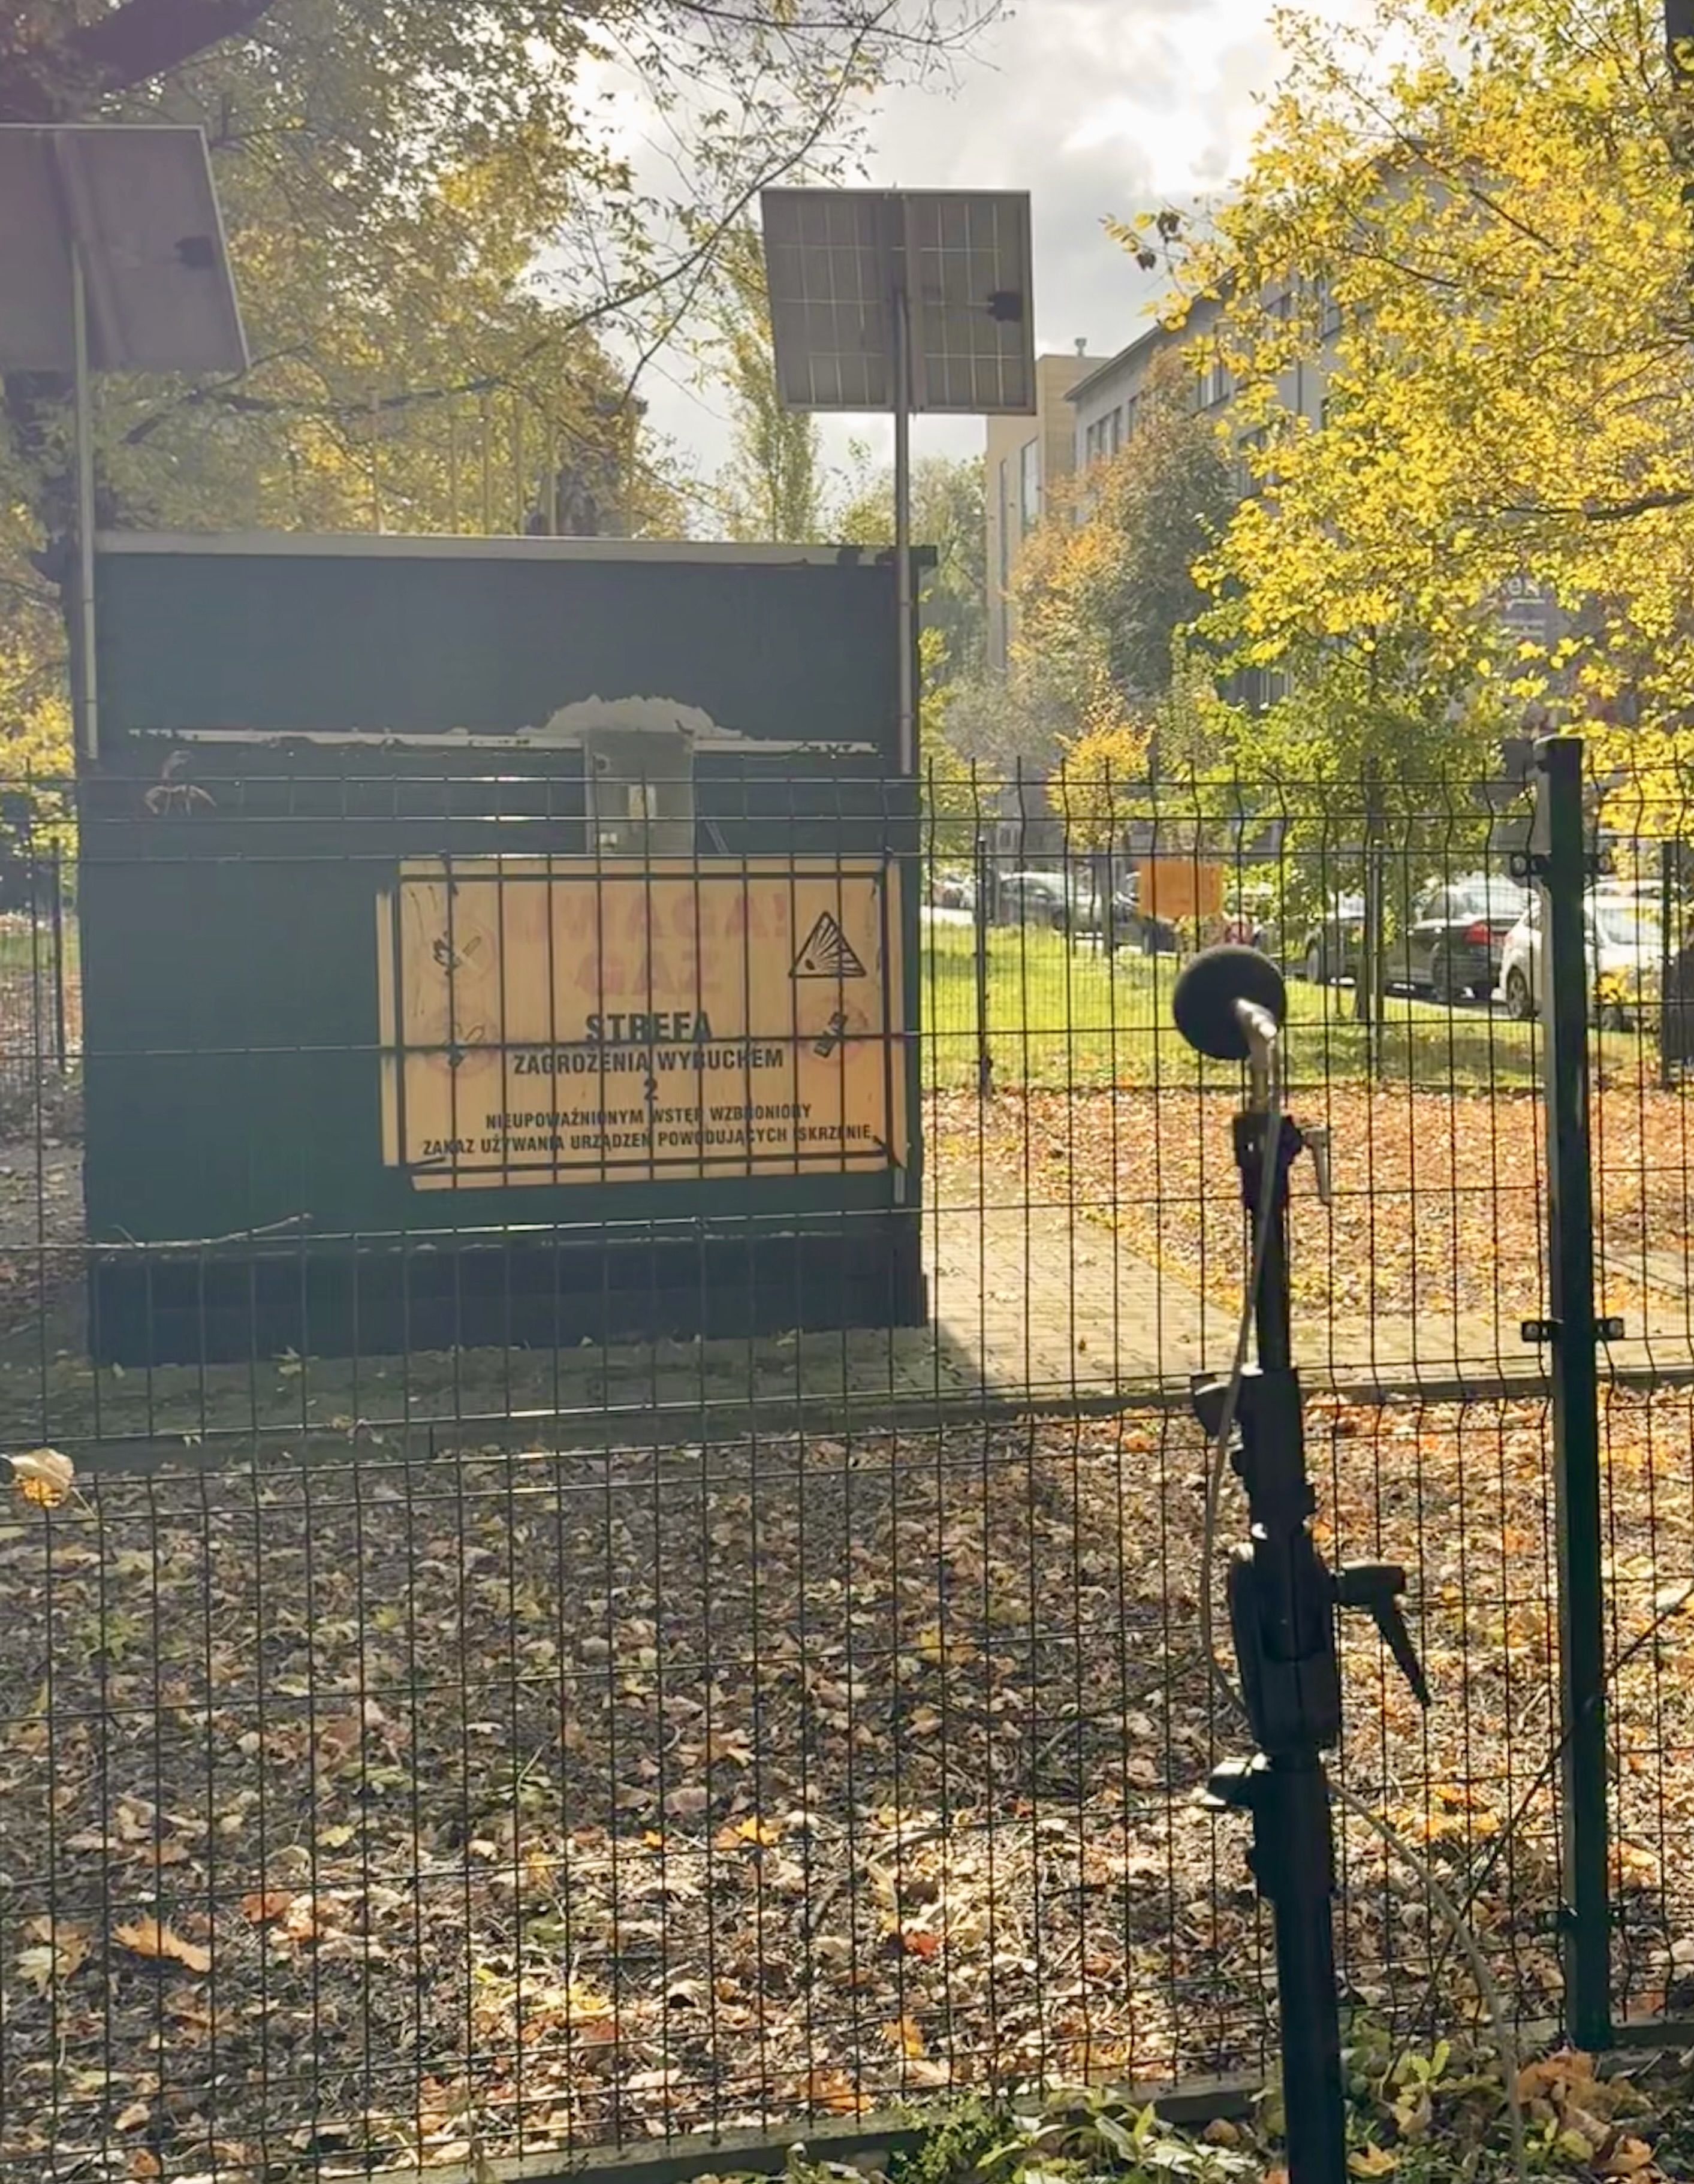
\includegraphics[width=0.5\linewidth,
        trim={0cm 10cm 5cm 30cm}, clip]{stacja_gazowa_mikrofon.jpeg}
    \caption{Stanowisko pomiarowe przy stacji gazowej nr 08/3159}
    \label{fig:stacja}
\end{figure}

\clearpage
\subsection{Charakterystyka otoczenia}
Według identyfikacji wykonanej podczas ćwiczenia stacja należy do
Polskiej Spółki Gazownictwa. Znajduje się na terenie zielonym,
w sąsiedztwie budynku Wydziału Inżynierii Środowiska i Geodezji
Uniwersytetu Rolniczego oraz ulic Oleandry i Romana Ingardena.
Ruch uliczny w pobliżu stacji stanowił potencjalne źródło zakłóceń w rejestrowanym sygnale. Nie dysponowano ilościowymi danymi o natężeniu ruchu.
Rozpatrywany w ćwiczeniu kierunek potencjalnej zabudowy nie stanowi
potwierdzenia przeznaczenia terenu w miejscowym planie
zagospodarowania przestrzennego.

\begin{figure} [H]
    \centering
    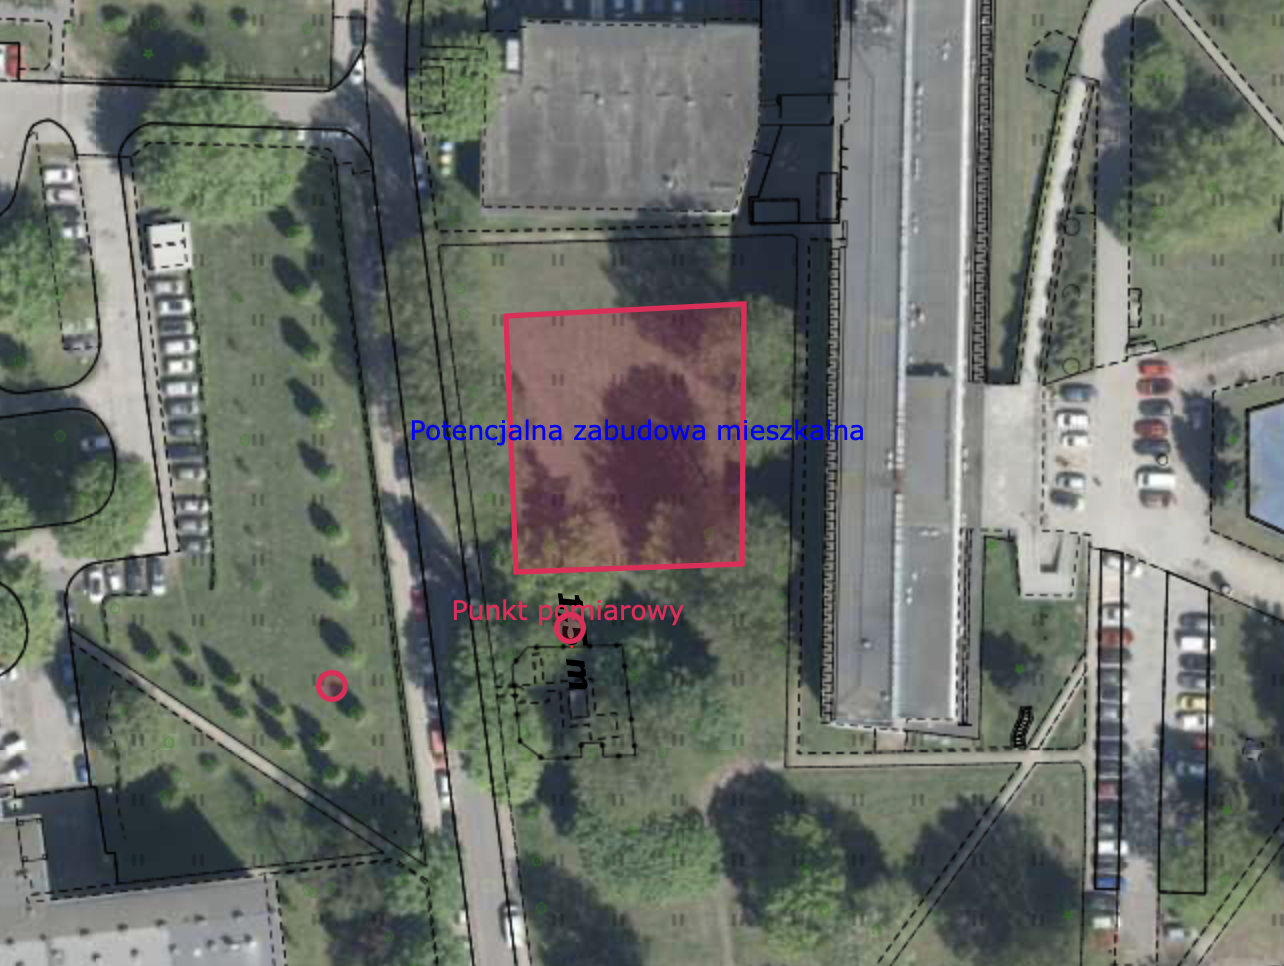
\includegraphics[width=0.5\linewidth]{potencjalna zabudowa.png}
    \caption{Usytuowanie stacji gazowej względem punktu pomiarowego i sąsiedniej zabudowy}
    \label{fig:otoczenie}
\end{figure}


\subsection{Lokalizacja punktów pomiarowych}
Punkt pomiaru hałasu zlokalizowano po północnej stronie stacji,
w odległości około $1{,}5\,\mathrm{m}$ od wskazanej podczas ćwiczenia
granicy obiektu. Mikrofon znajdował się na wysokości
$1{,}5\,\mathrm{m}$ nad gruntem. Punkt wybrano po stronie
rozpatrywanego kierunku potencjalnej zabudowy. Wynik charakteryzuje
to stanowisko; nie jest bezpośrednim pomiarem poziomu hałasu na
terenie odległej zabudowy.

\begin{figure}[H]
    \centering
    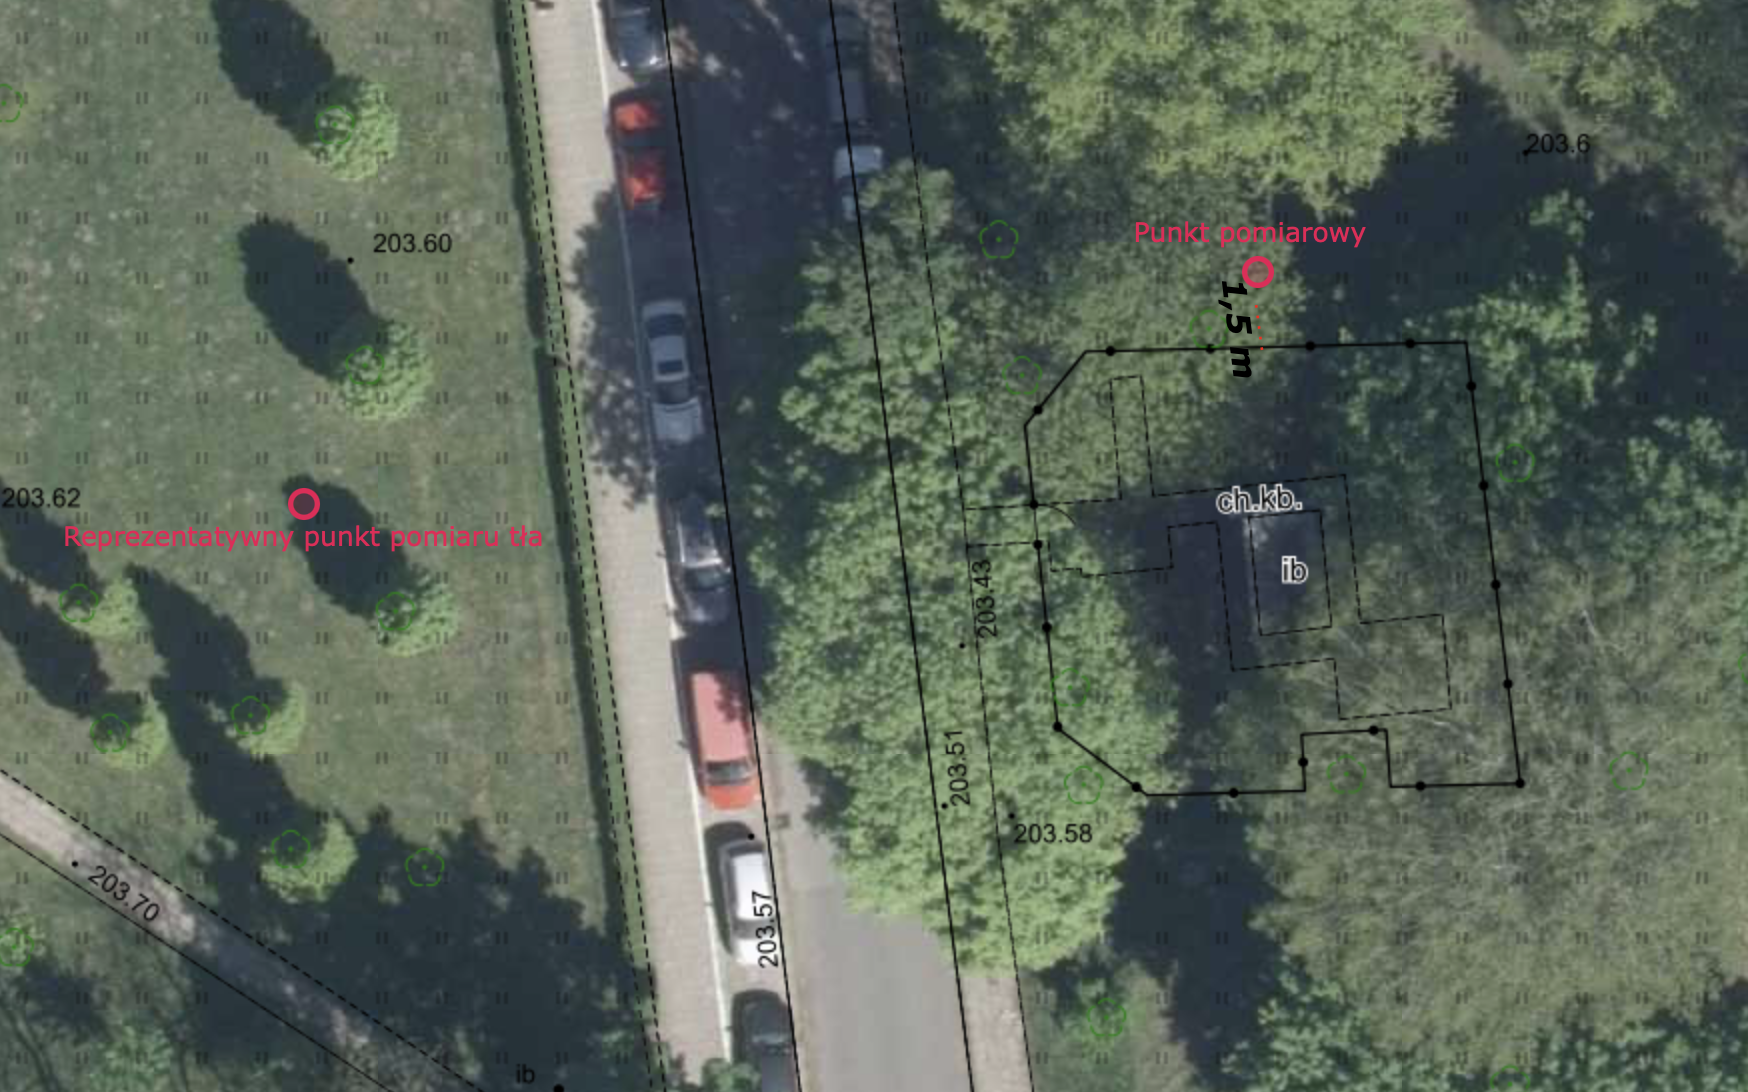
\includegraphics[width=0.8\linewidth]{punkty_pomiarowe.png}
    \caption{Lokalizacja punktu pomiaru hałasu oraz punktu pomiaru tła }
    \label{fig:punkty_pomiarowe}
\end{figure}

\subsection{Tło akustyczne}
Punkt pomiaru tła zaznaczono na rysunku~\ref{fig:punkty_pomiarowe}.
Ze względu na brak możliwości wstrzymania pracy stacji pomiar tła
wykonano w innym miejscu, po serii zasadniczej. Do pomiaru przy
stacji należą pliki P04--P08, a do pomiaru tła pliki P10--P14.
Nie udokumentowano ilościowo porównywalności oddziaływania źródeł
tła w obu punktach. Stanowi to ograniczenie interpretacji korekcji
tła akustycznego.
